%!TEX root = ../thesis.tex
% ******************************* Thesis Appendix B ********************************

\chapter{Notable results for stochastic dynamical systems}
\label{appresults}


This appendix puts together notable theoretical results for stochastic dynamical systems, that are of crucial importance to study systems' resilience and early warning signals. It is introduced by revising and exemplifying the concept of generic bifurcation, for their importance in the study of B-tipping. \\




\tocless\section{Generic bifurcations}
\label{sec:generic_bif}
As introduced in Def.~\ref{def:generic_bif}, a bifurcation is generic if it is not mapped onto another one after an unfolding (slight additive perturbation). Among low dimension bifurcations, fold and Hopf bifurcations are generic for codimension one \citep{kuznetsov2013elements}. In fact, the real part of an eigenvalue can reach zero (vanish) in two ways: either $\lambda = 0$ (appearance of a fold bifurcation), or a complex conjugate pair of eigenvalues reach the imaginary axis, $\lambda = \pm \omega_0 \, i$ (appearance of a Hopf bifurcation). The cusp bifurcation is generic for codimension two. Pitchfork and transcritical bifurcations are generic only if additional constraints about symmetry and asymptotic behaviour are considered, otherwise their unfolding maps them into a fold.

Envisioning realistic applications, when small perturbations or deviations from an ideal model are always present, the standard way of considering B-tipping is through the analysis of fold bifurcations and their associated early warning signals. Unless other types are considered for different scopes, the fold bifurcation is thus a good candidate to address local analysis and prediction of regime shifts driven by B-tipping mechanisms. To visualize this, consider a subcritical bifurcation (Fig.~\ref{fig:subpitch_bis}) and observe how its critical neighbourhood is locally mapped onto a fold after a small unfolding introduced by an additive parameter $q$, such that Eq. \ref{eq:subpitch} becomes $\dot{x} = px +x^3 +q$. 

\begin{figure}[h!]
	\centering
	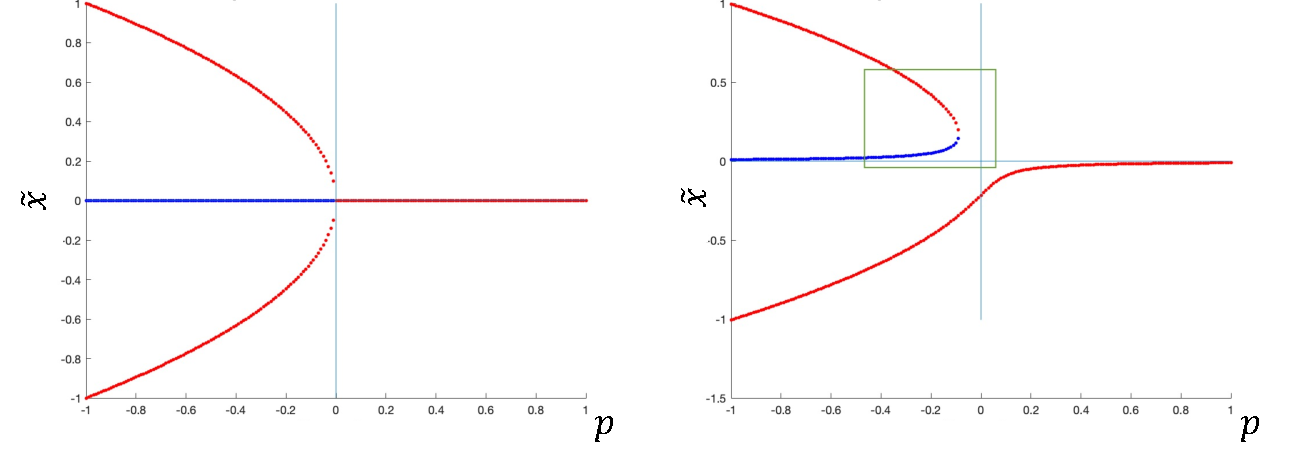
\includegraphics[width=0.7\linewidth]{unfolding}
	\caption{\small \textbf{Left:} bifurcation diagram of a subcritical pitchfork bifurcation \ref{eq:subpitch}. For better visualization, the vector field has been removed and the fixed equilibrium manifold coloured according to the stability of its points. Blue = stable; red = unstable. \textbf{Right:} bifurcation diagram of an unfolded subcritical pitchfork bifurcation $\dot{x} = px + x^3 + q$, where $q$ is the unfolding parameter. In this case, its value is fixed to $q = 0.01$ for visualization purposes. Note that locally (region highlighted by the green square) the bifurcation corresponds to a fold (\textit{cf.} Sec.~\ref{subsec:fold}).} 
	\label{fig:subpitch_bis}
\end{figure}




\tocless\subsection{Example: the Euler buckling problem}
An example of unfolding is the ``Euler buckling problem''. The swiss mathematician was the first to pose the following problem: imagine a slender, straight column sustaining a burden. What is its behaviour when the burden increases in weight? It was soon found that there exist a critical weight value that makes the column buckle. This behaviour, known as ``Euler's buckling'', is well known in engineering, including control engineering \citep{venkadesan2007manipulating}. For idealized slender columns, it is described with a subcritical pitchfork bifurcation \cite{thompson2011predicting,kuehn2013mathematical}. $\theta$ (angle of the column with respect to upright position) is the only degree of freedom available given the rotational invariance; $\mathcal{F_s}$ is the control parameter and is viewed as the force applied to the column. The model is \citep{venkadesan2007manipulating}:
\begin{equation}
	\dot{\theta} = p_1(\mathcal{F_s}-p_2)\theta + p_3\theta^3 - p_4\theta^5 \, ,
\end{equation}
where $p_i$ are additional parameters to be fixed.

\begin{figure}[h!]
	\centering
	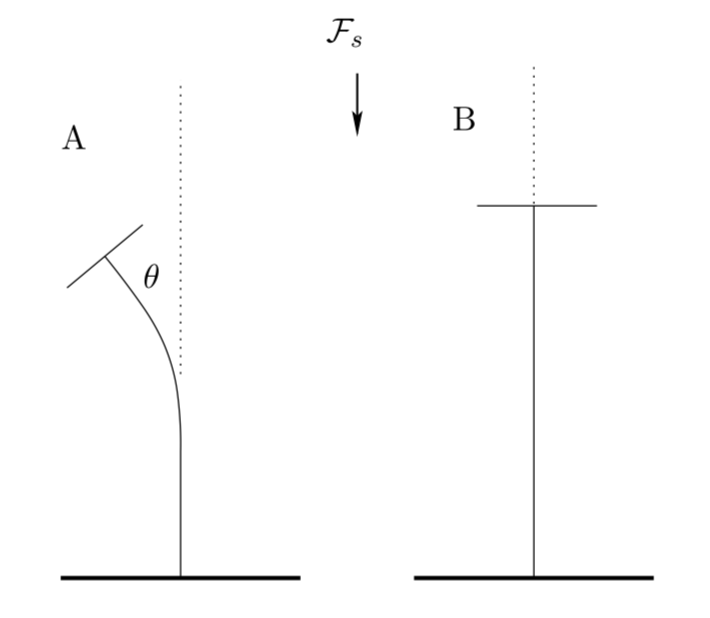
\includegraphics[scale=0.4]{buckling}
	\caption{Sketch of a column subjected to pressing force $\mathcal{F_s}$ \citep{kuehn2013mathematical}, eventually buckling. }
	\label{fig:buckling}
\end{figure}

When considering realistic columns, it is necessary to consider slight imperfections. This breaks the symmetry of the column, resulting in asymmetric buckling. Model-wise, these imperfections are inserted in the normal form as additive terms. The modified model is:
\begin{equation}
	\dot{\theta} = p_1(\mathcal{F_s}-p_2)\theta + p_3\theta^3 - p_4\theta^5 + q \, .
\end{equation}
$q$ is the unfolding parameter that destroys the bifurcation in a similar fashion to Fig. \ref{fig:subpitch_bis}, right. \\





\tocless\section{Ornstein-Uhlenbeck processes and critical slowing down}
\label{sec:o-u}

When studying critical transitions close to tipping points, Ornstein-Uhlenbeck (\gls{O-U}) processes (Eq. \ref{eq:o-u}) are of utmost importance to approximate their dynamics subject to small fluctuations. In fact, they correspond to continuous-time counterparts of autoregressive models, which are in turn the archetype of critical transition-prone systems, \textcite{Scheffer2009}. Overall, \gls{O-U} processes describe the motion of a particle moving in a quadratic potential with an escape barrier -- related to fold bifurcation normal form (\textit{cf.} Sec.~\ref{subsec:fold}) -- and subject to noise, that can model either random disturbances or  the action of fast degrees of freedom \citep{Berglund2006}. To recall the working hypothesis, they are:

\begin{enumerate}
	\item The system is evolving along the leading eigenvector of the bifurcation, that is, we are hypothesising a centre manifold setting. This modelling simplification holds as long as the system approaches a tipping point characterized by a shrinking manifold along the leading direction. This is also valid as long as we define a single macroscopic variable that accounts for a global mean field.
	\item Slowly varying parameter allowing the system to follow its changes adiabatically (slow-fast system and equilibrium hypothesis).
	\item Noise level is low, and a high signal-to-noise ratio is maintained. To begin with, let us consider additive white noise.
\end{enumerate}

To obtain the theoretical results leading to the existence and identification of early warning signals, hypothesis 1-3 must be satisfied. Relaxing one or more might yield different conclusions in the expected behaviour of \gls{EWS} (see Chapter ~\ref{ch:EWS_sensitivity}). 

Historically, Ornstein-Uhlenbeck processes have been deeply studied and many results and demonstrations are available in books covering stochastic processes (e.g. \textcite{Allen2014,Gardiner1985,Berglund2006,Risken1991,papoulis2002probability}). Hence, this section concentrates on results that are of direct relevance for the current development of the \gls{CT} framework, while further reading is directed to the books just mentioned.

\tocless\subsection{Studying how perturbations evolve in B-tipping driven by a fold}
Recall the normal form of a generic fold bifurcation, Eq.~\ref{eq:fold}:
\begin{equation}
	\dot{x} = p+x^2 \, ,
	\label{eq:nf}
\end{equation}
It has two steady states:
\begin{equation}
	\hat{x_1} = -\sqrt{-p - 0} \; \; \text{(stable)}
	\label{eq:stable}
\end{equation}
\begin{equation} \label{eq:stability_fold}
	\hat{x_2} =-\sqrt{-p - 0} \; \; \text{(unstable)}
\end{equation}
where the term ``$-0$'' explicits the distance from the saddle point that, from the properties of the normal form, is located in $x_c = 0$. Let us now ``sit'' in a neighborhood of the attractor (stable fixed point) $\hat{x_1}$ to see what happen after small perturbations. Hence, we perform a local linearization by considering $\delta x = (x - \hat{x}_1)$. Thus:
\begin{equation}
	\frac{d \delta x}{dt} \simeq f(\hat{x}_1) + \frac{\partial f}{\partial x}|_{\hat{x}_1} \delta x + \mathrm{O}(\delta x^2) \, .
\end{equation}
So, using Eq. \ref{eq:nf} and Eq. \ref{eq:stable}, we obtain:
\begin{equation}
	\frac{d \delta x}{dt} \simeq 2 \sqrt{-p} \delta x \, .
\end{equation}
Let us now convert this deterministic form into a stochastic one by adding a Wiener process with diffusion term $\sigma$. This modelling choice converts the family of \gls{ODE}s into \gls{SDE}s. Here, we skip some mathematical formalism, which has been covered during the years by \textcite{khas1966limit}, \textcite{namachchivaya1990equivalence} and \textcite{Berglund2006} among the others, and concentrate on the physical interpretation. In addition, a change $\delta x \rightarrow y$ makes the notation lighter into:
\begin{equation}
	dy = 2\sqrt{-p} y \, dt + \sigma dW \, .
	\label{eq:langevin}
\end{equation}
The equation describes a system evolving under small noise in a neighbourhood of the stable equilibrium, when this is not far away from the saddle node (linearization). An illustrative sketch is presented in Fig. \ref{fig:sketch_fold_noise}. 

\begin{figure}[h!]
	\centering
	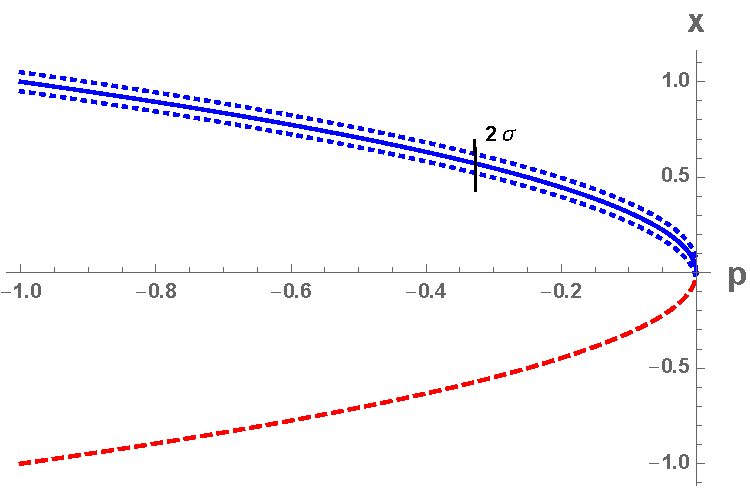
\includegraphics[width=0.4\linewidth]{saddle_node}
	\caption{\small Bifurcation diagram of the saddle-node, with uncertainty band given by the noise level}
	\label{fig:sketch_fold_noise}
\end{figure}

The term $(\hat{x_1} - 0) = \sqrt{-p}$ is precisely the distance of the stable equilibrium from the saddle node and depends on the leading parameter $p$. From now on, we rescale it to a new variable $-k$. 
\begin{equation}
	dy = -k \, y \, dt + \sigma dW
	\label{eq:OU}
\end{equation}
The sign $``-''$ in $``-k''$ is inserted to be consistent with the following interpretation: Eq. \ref{eq:OU} is the associated Langevin equation to a Ornstein-Uhlenbeck process (compare with Eq. \ref{eq:o-u} and see \textcite{papoulis2002probability, Gardiner1985}). 

Consequently, we can interpret the term that multiplies the deterministic drift as $-\frac{\partial V}{\partial x}$ where $V(x)$ is the potential governing the drift of the particle subjected to random noise. In our case, thanks to the choices made, 
\begin{equation} \label{eq:potential_fold}
	V = \frac{1}{2} k \, y^2 \, ,
\end{equation}
that is, a quadratically shaped adjoining potential typical of an overdamped oscillator under noise, of which $k$ represents the depth. The quadratic potential can be termed differently, according to the points of view of different sub-fields: ``effective potential'' in nonequlibrium phase transitions \citep{zaikin2001additive}, ``quasi-potential'' in large deviation theory \citep{freidlin1998random,Nolting2016,Zhou2012}. The working hypothesis is that boundary of the ideal potential $V$ can grasp the boundary of the attracting basin of the original model after sufficiently long time. Hence, it proves to be analytically tractable and presents the necessary steps to understand the main qualitative features of more complicated critical transitions. However, it requires ad hoc extensions when studying system-specific quantitative details like observability boundaries and lead times.

Given the relationship $k = 2(0 + \sqrt{-p})$ from Eq. \ref{eq:langevin}, when the equilibrium approaches a saddle point ($p$ goes towards zero from negative values) the associated analytical potential gets flatter as $k$ approaches zero, see also Fig. \ref{fig:fold_diag} (centre). Intuitively, recall the ``pebble-down-the-hill'' analogy (Sec.~\ref{subsec:pebble}). The potential governs the acceleration under which a rolling ball moves; hence, it is connected to the recovery time after a perturbation that moves the ball away from the equilibrium. When the system approaches its saddle node, the recovery time slows down. Thus we get the phenomenon of Critical Slowing Down \gls{CSD}. The scaling of slowing down depends on the specific dependence of $k$ to $p$. For a fold, it goes as a square root; or other bifurcations, it might vary (see sections above). 

Thanks to the discussed methodology, we can now study saddle-node driven B-tipping using the formalism of Stochastic Processes, where the potential depth (at quasi-steady state) plays the role of the control parameter. In the remaining of this section, the general distance-to-critical-point $k$ will be employed. For each specific bifurcation, it will suffice to substitute the dependence $k = k(p)$ (see also \textcite{Kuehn2011}) to get the correct scaling of each notable characteristic (statistical indicators, power spectrum, etc.). Estimating the scaling of observed regime shifts has been proposed as a notable feature to distinguish the (potentially) underlying bifurcations \citep{Meisel2012a,Bury2020}. \\


\tocless\subsection{Critical Slowing Down (CSD)}
\label{subsec:CSD}

In statistical mechanics, \gls{CSD} is a phenomenon connected to second-order phase transitions. At the equilibrium point, decays of small perturbations are slower, as they follow lower order polynomials \cite{strogatz2018nonlinear}. First-order phase transitions, which are in turn related to critical transitions, are also affected by \gls{CSD} when approaching a tipping point. Let us first concentrate on critical slowing down in fold transitions (around saddle-node points). According to centre manifold theory, it is sufficient to study the behaviour of the vector field in a neighbourhood of the tipping point in order to inquire the relaxation coefficient (often called Lyapunov coefficient, \textcite{Kuehn2011}).

Similarly to the subsection above, we begin from the normal form Eq. \ref{eq:nf} and concentrate around the stable equilibrium point $\hat{x}_1$. Let us consider small deviations $y$ around $\hat{x}$. For sufficiently small deviations, they are described by a linearization $\dot{y} = f(\hat{x}+y)-f(\hat{x}) \, y \simeq (D_x f)|_{\hat{x}} \, y$, where $f(x)$ is the vector field (right hand term in Eq. \ref{eq:OU}). Therefore, for the fold we get:
\begin{equation}
	u' = -2x|_{\sqrt{-p}} \, u= -2\sqrt{-p}u
\end{equation}
Hence, any perturbation decays as $O(-p^{1/2})$ back to the equilibrium, with a relaxation coefficient is $\alpha = 1/2$. Determining the relaxation coefficients for other bifurcations allows assessing their CSD scaling (reported in Sec.~\ref{sec:normal_form} or each normal form). \\


\tocless\subsection{Stochastic indicators towards tipping points}
\label{subsec:stocastii_EWS}
In an Ornstein-Uhlenbeck process, the drift coefficient (distance to tipping) can be interpreted as the potential depth, and is thus immediately related to system's resilience. As the trends of statistical indicators of \gls{O-U} processes is known to depend on the drift term, it is also immediate to study how such trends change when the leading parameter is varied. The corresponding results have been proposed to provide early warning signals for an impending shift. Let us express Eq. \ref{eq:OU} using another typical notation for stochastic processes, $y_t = y(t)$ and $\sigma = \sqrt{2D}$.
\begin{equation}
	dy_t = -k \, y_t \, dt + \sqrt{2D} dW_t
	\label{eq:OU-ok}
\end{equation}
The statistical indicators of the stationary process\footnote{A stochastic process is said to be \textit{stationary} if its mean does not depend on time ($\text{mean} = \eta = \text{const}$) and its covariance only depends on time differences: $\langle x(t)x(t') \rangle$ = $\langle x(t)x(t+\tau) \rangle$, where $\tau = t' - t$.} Eq. \ref{eq:OU-ok} are derived as \citep{papoulis2002probability,Gardiner1985}:
\begin{itemize}
	\item Covariance (temporal self-correlation): $\langle y_t y_{t'} \rangle = \frac{D}{k}e^{-k|t-t'|} $.
	\item Variance: $\langle y_t^2 \rangle - \langle y_t \rangle ^2 = \frac{D}{k}(1-e^{-2kt})$. Hence, for $t \to \infty$, 
	\begin{equation}
		Var \xrightarrow[]{t \to \infty} \frac{D}{k}
	\end{equation}
	\item Autocorrelation: $e^{-k|t-t'|}$. Hence, 
	\begin{equation}
		\gls{AC(1)} = e^{-k}.
	\end{equation}
	\item In general, all other statistical moments can be expressed as:
	\begin{equation}
		\langle y^n \rangle - \langle y \rangle^n = \int_{-\infty}^{\infty} (y'-\mu)^nP(y')dy' 
	\end{equation}
	where $P(x)$ is the probability density function, a Gaussian in case of white noise or derived from the Fokker-Plank equation (see Sec.~\ref{sec:fokker_plank}), and $\mu$ is the mean expected value.
	\item Power spectral density: 
	\begin{equation}
		S(\omega) = \frac{D}{\pi(k^2 + \omega^2)}
	\end{equation}
	\item Shannon entropy:
	\begin{equation}
		H_s(y)  = \frac{1}{2} \log(2 \pi \text{Var}) + 1
	\end{equation}
\end{itemize}
Additional entropy and auto-information measures can be further derived for other processes obeying other evolution laws \citep{Frank2004,Heseltine2016,Heseltine2019,Chapeau-Blondeau2007} or being analysed with diverse orthogonal basis like wavelets \citep{Coifman1992,Kirby2005,Abdel-Hamid2016}.

\begin{proof}
	Proof for Variance, Covariance and Autocorrelation. Equation \ref{eq:OU-ok} is solved with an Itô-like integration and the method of constants for differential equation solution :
	\begin{enumerate}
		\item Ansatz of solution: $z = y_t \, e^{kt}$
		\item Itô differentiation: 
		\begin{align*} 
			d \left( e^{kt} y_t \right) &= k \, e^{kt} y_t \, dt + e^{kt} dy_t \\ 
			&= ke^{kt} y_t \, dt + e^{kt} \left( -k \, y_t \, dt + \sqrt{2D} \, dW_t \right)	\\
			&= e^{kt} \, \sqrt{2D} \, dW_t \, .
		\end{align*}
		\item Integration and re-substitution for $z$
		\begin{equation} \label{eq1}
			\begin{split}
				e^{kt} y_t - y_0 & = \sqrt{2D} \int^t_0 e^{sk} dW_s \\
				y_t & = y_0 e^{-kt} + \sqrt{2D} \int_{0}^{t} e^{k(s-t)} dW_s \, .
			\end{split}
		\end{equation}
		This is the stochastic trajectory.
	\end{enumerate}
	If the initial condition is deterministic or Gaussian, it is straightforward to estimate mean and time correlation function:
	\begin{align*}
		\langle y_t \rangle &= \langle y_0 e^{-kt} + \sqrt{2D} \int_{0}^{t} e^{k(s-t)} dW_s \rangle && \text{\textbf{Mean}}\\
		&= \langle y_0 e^{-kt}  \rangle + \langle  \sqrt{2D} \int_{0}^{t} e^{k(s-t)} dW_s \rangle \\
		&= y_0 e^{-kt} + \sqrt{2D} \int_{0}^{t} e^{k(s-t)} \langle dW_s \rangle \\
		&= y_0 e^{-kt} + 0 \xrightarrow[]{t \to \infty} 0
	\end{align*}
	\begin{align*}
		\langle y_t y_{t'} \rangle &= y_0^2 e^{-k(t-t')} + \left( \sqrt{2D} \right) ^2 \int_{0}^{t} \int_{0}^{t'} e^{k(s-t)} e^{k(s'-t')} \langle dW_s \, dW_{s'} \rangle && \text{\textbf{Covar.}}\\
		&= y_0^2 e^{-k(t-t')} + 2D \, e^{-k(t+t')} \int_{o}^{t} \int_{0}^{t'} e^{k(s+s')} \delta(s-s') \, ds \, ds'
	\end{align*}
	where we used the property of Wiener processes $ \langle dW_s \, dW_{s'} \rangle = \delta(s-s') \, ds \, ds' $. $\delta(s-s')$ is the Dirac delta. Then:
	\begin{align*}
		\langle y_t y_{t'} \rangle &=  y_0^2 e^{-k(t+t')} + 2D \, e^{-k(t+t')} \left. \frac{e^{2k - min(s,s')}}{2k} \right\rvert_0^{min(t,t')}\\
		&=  y_0^2 e^{-k(t+t')} + \frac{D}{k} e^{-k(t+t')} \left( e^{2k - min(t,t') } -1  \right) \\
		&= y_0^2 e^{-k(t+t')} + \frac{D}{k}e^{-k|t-t'|} - \frac{D}{k}e^{-k(t+t')} \, .
	\end{align*}
	By neglecting the rapid initial transient, we finally get:
	\begin{equation} \label{eq:covar}
		\langle y_t y_{t'} \rangle  \xrightarrow[]{t,t' \to \infty} \frac{D}{k}e^{-k|t-t'|} 
	\end{equation}
	
	Finally, to estimate the \textbf{variance}, use its definition:
	\begin{equation} \label{eq:variance}
		\langle y_t^2 \rangle - \langle y_t \rangle ^2 = \langle y_t y_{t'} \rvert_{t'=t} \rangle -  \langle y_t \rangle ^2 = \frac{D}{k} \left( 1- e^{-2kt} \right)
	\end{equation}
	
	The \textbf{autocorrelation} follows as:
	\begin{equation} \label{eq:autoc}
		Autoc = \frac{Cov(x(t) x(t'))}{\sqrt{Var(x(t)) Var(x(t'))}} = e^{-k \cdot |t-t'|} \; \text{for} \; t,t' \to \infty
	\end{equation}
\end{proof}

\begin{proof}
	Proof for the power spectral density $S(\omega)$. 
	
	In a stationary stochastic process, its spectral density is defined as the Fourier transform of the Covariance function \cite{papoulis2002probability}:
	\begin{equation}
		S(\omega) = \mathcal{F}\left[ E\left\{ y(t+\tau)y(t)  \right\}  \right] = \frac{1}{2 \pi}\int_{-\infty}^{\infty}R(\tau)e^{-i\omega t} dt
		\label{eq:spectrum}
	\end{equation}
	where $R(\tau)$ is the covariance function and the dimension of the spectral density is $\left[S(\omega) \right] = \text{dB}$. In case $t,t' \to \infty$ we already have the expression for the covariance function (Eq. \ref{eq:covar}), so the calculation is straightforward as long as we perform a change of coordinates $|t'-t| \rightarrow |t|$ which is valid for stationary processes:
	\begin{align*}
		S(\omega) &= \frac{1}{2 \pi} \int_{-\infty}^{\infty} e^{-i \omega t} \frac{D}{k} e^{-k|t|} \\
		&= \frac{D}{2 \pi k} \left(\int_{-\infty}^{0} e^{t(-i\omega + k)} dt + \int_{0}^{\infty}e^{-t(i\omega +k)} dt \right) \\
		&= \frac{D}{2 \pi k} \left( \frac{1}{-i\omega + k} + \frac{1}{i\omega +k}   \right) \\
		&=\frac{D}{\pi k}\frac{k}{k^2 + \omega^2}
	\end{align*}
	So the final expression is: 
	\begin{equation}
		S(\omega) = \frac{D}{\pi(k^2 + \omega^2)}
	\end{equation}
	
	Alternatively, we can consider the \gls{O-U} process as a stochastic input process with $R_{xx}(\tau) = q \delta(\tau)$ (white noise input) and linear transfer function $h(\tau)$ given by $h'(\tau) + ch(\tau) = \delta(\tau)$ (linear response given by potential). Then, in Fourier space,
	\begin{equation*}
		S_{yy} = q \frac{1}{k^2 + \omega^2}
	\end{equation*}
	where $q = D/\pi$ and $c = k$ (from the potential).
\end{proof}


\begin{proof}
	Proof for the Shannon entropy of a stationary process subject to Gaussian noise.
	
	Consider a Gaussian distributed variable $y \sim \mathcal{N}(\mu, \text{Var})$. Its entropy is:
	\begin{align*}
		H_s(y) & = - \int p(y')\log p(y')dy' =  \\
		& = - \mathbb{E}\left[ \log \mathcal{N}(\mu, \text{Var})  \right] =\mathbb{E} \left[ \log \left[ \frac{1}{\sqrt{2 \pi \text{Var}}} \exp \left(-\frac{1}{2 \text{Var}}(x-\mu)^2 \right)  \right]  \right] = \\
		& = \frac{1}{2}\log\left(2\pi\text{Var}\right) + \frac{1}{2\text{Var}}\mathbb{E}\left[(x-\mu)^2\right] = \\
		& = \frac{1}{2}\left( \log (2 \pi \text{Var}) +1 \right)
	\end{align*}
	
\end{proof}

Eq. \ref{eq:covar} and \ref{eq:variance} express how covariance and variance evolve when a quasi-steady parameter shapes the potential towards a tipping point. The limit $t,t' \rightarrow \infty$ is representative of system timescales that are much longer than that of the noise (the system relaxes to its equilibrium). It is possible to recognize an increase in both measurements when $k \to 0$. This phenomenon, illustrated in Fig. \ref{fig:ews_theo}, was suggested by \textcite{scheffer2009early} as an early warning signal (\gls{EWS}) to detect the approach towards a tipping point. Since the spectral density also depends on $k$, it can also be studied to suggest other early warning signals, as well as entropy measures.


\begin{figure}[h]
	\centering
	
	\begin{minipage}[c]{0.47\textwidth}
		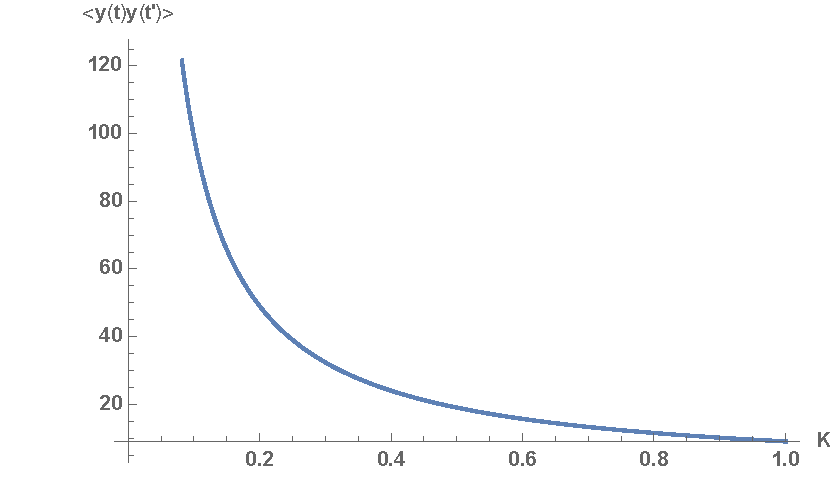
\includegraphics[width=0.85\linewidth]{autocorr_1}
		\renewcommand{\figurename}{Fig.}
	\end{minipage}
	\hspace{0.01cm}
	\begin{minipage}[c]{0.47\textwidth}
		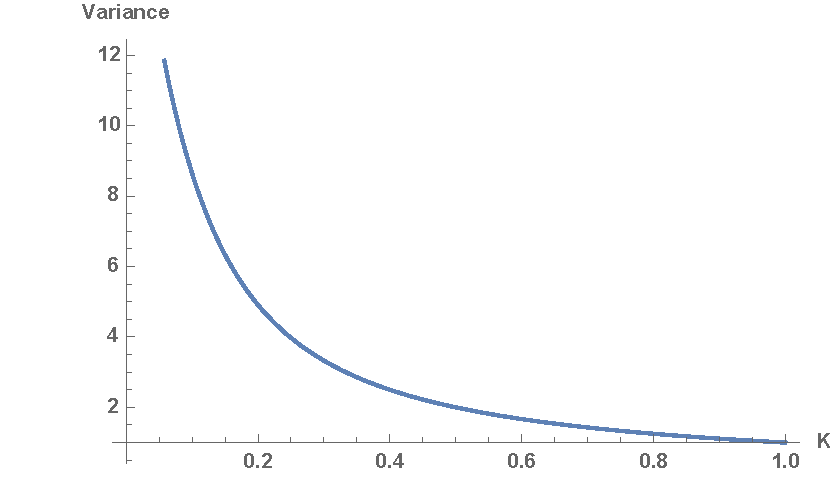
\includegraphics[width=0.85\linewidth]{var}
		\renewcommand{\figurename}{Fig.}
	\end{minipage} 
	
	\caption{\small \textbf{Left:} Covariance, with $\delta t = 1$, vs parameter $k$. \textbf{(Right)} Variance vs $k$. Note that both measures increase when $k \to 0$. Such an increase has been suggested to provide an early warning signal.}
	\label{fig:ews_theo}
\end{figure}

\begin{figure}[h]
	\centering
	
	\begin{minipage}[c]{0.47\textwidth}
		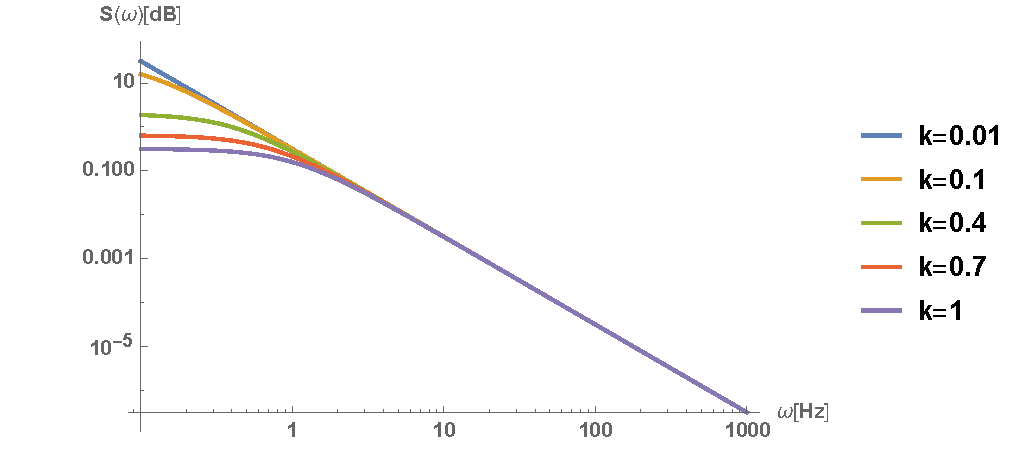
\includegraphics[width=0.9\linewidth]{spectrum}
		\renewcommand{\figurename}{Fig.}
	\end{minipage}
	\hspace{0.01cm}
	\begin{minipage}[c]{0.47\textwidth}
		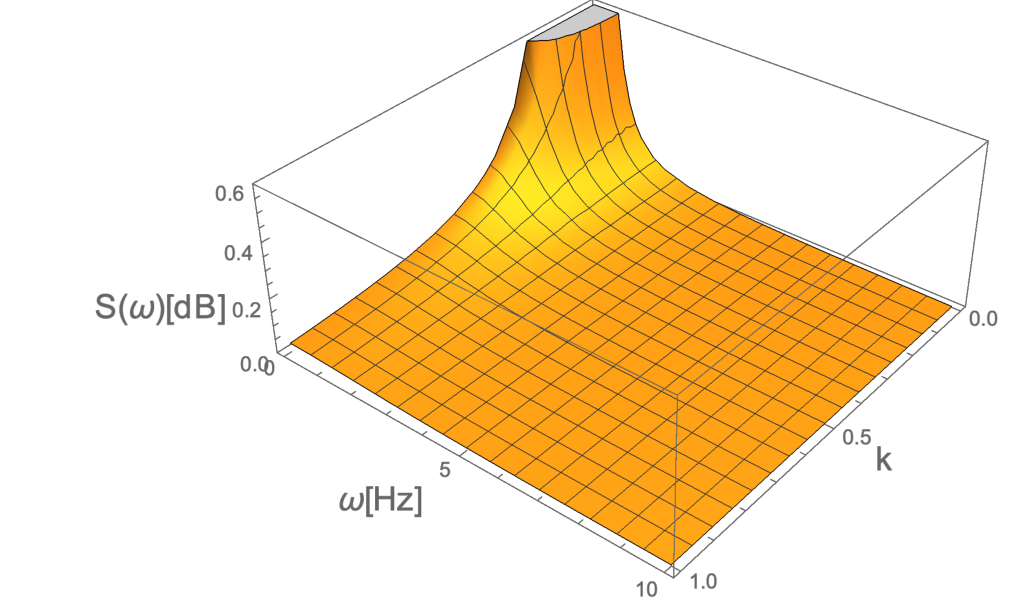
\includegraphics[width=0.9\linewidth]{spectrum_surface}
		\renewcommand{\figurename}{Fig.}
	\end{minipage} 
	
	\caption{\small \textbf{Left:} Power spectral density for frequencies $\omega$, at different values of the parameter $k$. The reddening (increasing power on low frequencies) happening for decreasing $k$ has been associated to potential \gls{EWS} \citep{thompson2011predicting,biggs2009turning}. \textbf{Right:} Full dependency of $S(\omega,k)$ on both $\omega$ and $k$, provided that the latter is varied at quasi-steady sate and hat the process is overall stationary.}
	\label{fig:spectral_reddening}
\end{figure}


From the theoretical derivation of early warning signals, one immediately recognise some important features that have been studied more in detail in recent computational works, i.e. \citep{kuehn2013mathematical,dessavre2019problem,brett2017anticipating,o2018stochasticity} and assessed against empirical data in \citep{proverbio2022performance}. The variance is generally more ``stable'' than covariance and autocorrelation against the choice of a moving window, as it does not depend on a $\delta t = |t-t'|$. As shown in Fig.~\ref{fig:covar_delta}, for higher $\delta t$, the time correlation remains flat for wider intervals of $k$, but then increases more rapidly. This induces a tradeoff between its sensitivity (how big its differential change is, which is related to how well we can discriminate between a real signal and a sampling of noise) and the predictability lag (how far from the critical value it is possible to determine an increase). On the other hand, the autocorrelation does not depend explicitly on the noise distribution and is thus insensitive to its details, contrary to the variance. 

These characteristics hold as long as we have repeated measurements over an ergodic distribution. The assumption of ergodicity\footnote{An ergodic system is such if the mean over repeated measurements equals the mean over time.} might be true if we allow the system to relax back to its equilibrium, that is, $k$ is almost fixed with comparison to the system timescale and the measurement rate. However, a sliding window technique might yield invalid estimates if the ergodic assumption is not valid.


\begin{figure}[h!]
	\centering
	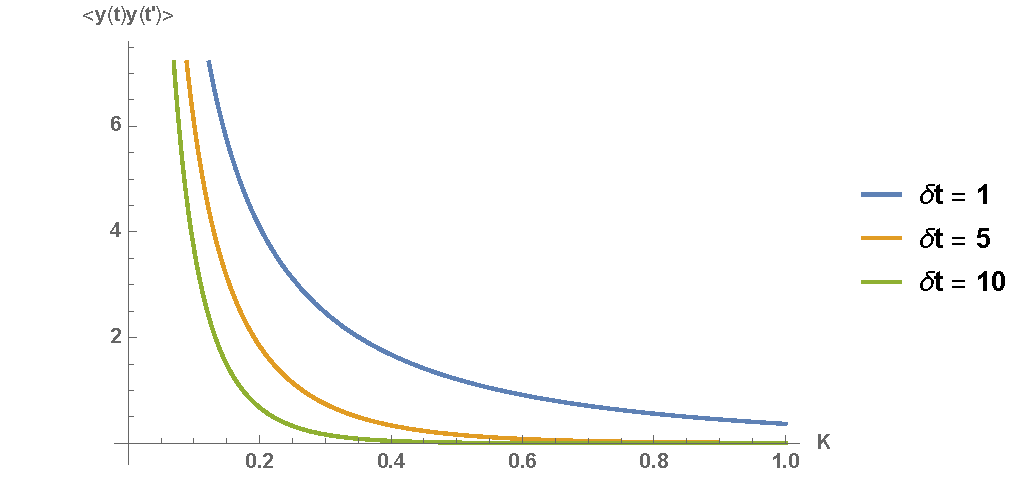
\includegraphics[width=0.5\linewidth]{autocorr_deltat}
	\caption{\small Temporal correlation vs $k$ at different $\delta t$: $\langle y(t)y(t+\delta t) \rangle$. }
	\label{fig:covar_delta}
\end{figure}



\tocless\section{Fokker-Plank equation and stationary probability density functions}
\label{sec:fokker_plank}

The Fokker-Planck equation \ref{eq:fokker_plank} describes the evolution of the probability density function $P(x,t|x_0,t_0)$ that a process takes the value $x$ at time $t$, from its previous state. Let us recall it here:
\begin{equation}
	\partial_t P(x,t | x_0, t_0) = - \partial_x \left[A(x,t) P(x,t | x_0, t_0) \right] + \frac{1}{2} \partial^2_x \left[B(x,t)^2 P(x,t | x_0, t_0) \right]
\end{equation}
 From now on, the terms ``$|x_0,t_0$'' will be implied. Solving the Fokker-Planck provides information about the full evolution of $P(x,t)$, which is paramount to estimate statistical moments for the whole process as \citep{papoulis2002probability}:
\begin{equation}
	\mathbb{E}[h(x)] = \int_{x}^{\infty} h(x') P(x') dx' 
\end{equation}
where $\mathbb{E}[\cdot ] $ denotes the expected value. 


Solving the Fokker-Plank equation might be complicated, depending on the specific shape of $A(x,t)$ and $B(x,t)$. For stationary processes and for differentiable and integrable functions, it is instead possible to estimate the stationary probability density function (\gls{SPDF}) by solving $\partial_t P(x,t) = 0$ as \citep{Risken1991}:
\begin{equation}
	P_s(x) = \frac{N_c}{B(x)}\exp\left(\int^x \frac{A(x')}{B(x')} dx' \right) \, .
\end{equation}
$N_c$ is a normalization constant to interpret $\int P_s(x') dx'$ as a probability. $P_s(x)$ can also be put in the form:
\begin{equation}
	P_s(x) = N_c e^{-\phi(x)} \, . 
\end{equation}
Here, $\phi(x)$ is called the stochastic potential of the system. This function maps the equilibria of the stochastic dynamical system and their basins of attraction, allowing an interpretation of ``pebble down the hill'' for the asymptotic behaviour of the system. It thus reconstructs the ``adjoint''/''effective''/``quasi-'' potential introduced before, starting from the \gls{PDE} associated to the considered system. Application examples include \citep{Sharma2016,Su2019}. \\



\tocless\section{Kramers' escape rate and mean first passage times}
\label{subsec:kramer}
Essentially, the idea behind early warning signals for critical transitions is: given a stochastic process, how do its statistical indicators change when the underlying potential is varied under the influence of a leading parameter? 

As a consequence, one can use the manifold results in stochastic processes theory, analyse their dependence on parameters and interpret them accordingly. Two additional measures that provide insights onto the behaviour of stochastic dynamical processes are the mean first passage time (\gls{MFPT}) and the Kramers' escape rate. In escape problems from a potential well, they respectively measure how long a system is expected to jump onto an alternative equilibrium for the first time, or how often the system is expected to reach the top of the potential barrier. Since they are directly related to probabilities of shifting equilibria, both the \gls{MFPT} and the Kramers' rate have been proposed as measures of system's resilience \citep{Sharma2016,Arani2021}.  Like above, this section provides an overview of salient features for both measures. Further reading and proofs can be found in \textcite{van1992stochastic} and \textcite{Gardiner1985}. \\

Consider a double-well potential like that in Fig. \ref{fig:double_well}. Assume it is (locally) quadratic near the attractor and (locally) quadratic around the barrier tip. Also assume we work in the damped regime and thus we can write the stochastic dynamics as a Langevin equation. Because of noise, the system can fluctuate away from the equilibrium (point $a$) and reach the top of the barrier (point $b$) by chance. From there, it can rapidly fall into a new attracting state. As above, we work with the ergodic hypothesis that the average time evolution of a system equals its statistical repetitions. Another assumption is that the well is deep compared to noise level. The rate at which many copies of the system can reach the potential top, in a stationary process at equilibrium under Gaussian noise and in time-independent potential, is solved by Kramers' escape problem \citep{van1992stochastic}. A clear derivation, accounting for each assumption presented above, is provided by \textcite{ritchie2016early}. As a bottom line, the Kramers' escape rate, for any left(right)-adjointed potential, is given by:
\begin{equation} \label{eq:kramers}
	\langle T(y) \rangle \simeq 2 \pi \frac{e^{\frac{V(b) - V(a)}{D}}}{\sqrt{V''(a) |V''(b)|}}
\end{equation}
where $V''$ denotes second derivate and $a$ and $b$ are, respectively, the point of potential minimum and maximum. Recall that, in this section, the variable $y$ denotes the local linearization next to a quadratic potential.


\begin{figure}[h!]
	\centering
	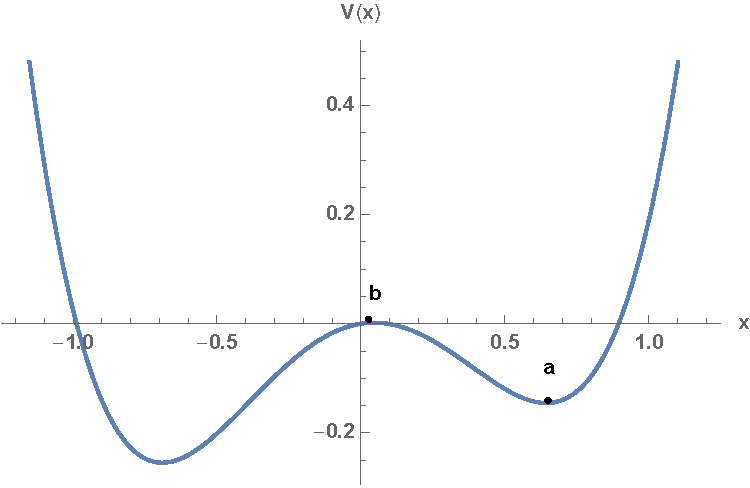
\includegraphics[width=0.4\linewidth]{double_potential}
	\caption{\small Representation of a double-well potential.}
	\label{fig:double_well}
\end{figure}


In case of \gls{O-U} process, associated to a linearised approach to saddle-node, evaluating the mean Kramers' escape rate $\langle T(y) \rangle$ vs the parameter $k$ is straightforward. $k$ represents both the potential height difference and its second derivative nn the equilibrium points (see Eq. \ref{eq:potential_fold} and substitute Eq. \ref{eq:stability_fold} into it.). Thus, by substituting $k$ into Eq. \ref{eq:kramers}, we get:
\begin{equation} \label{eq:exit_time}
	\langle T(y) \rangle \simeq \frac{2 \pi}{ k} e^{\frac{-k}{D}}
\end{equation}
where the absolute value is dropped since $k \in \mathbb{R}_+$. Fig.~\ref{fig:kramers} shows how the escape rate changes according to $k \to 0$ and for different levels of noise intensity $D$. The mean escape rate of particles flowing from the original well increases rapidly as the tipping point is approached. With high noise, $\langle T(y) \rangle$ is already non-zero even for large $k$, which is indicative of the N-tipping phenomenon. Therefore, provided that abundant measures and prior knowledge of noise levels are available, the mean escape rate can be used as a proxy for the potential depth and thus for the system's resilience.

\begin{figure}[h!]
	\centering
	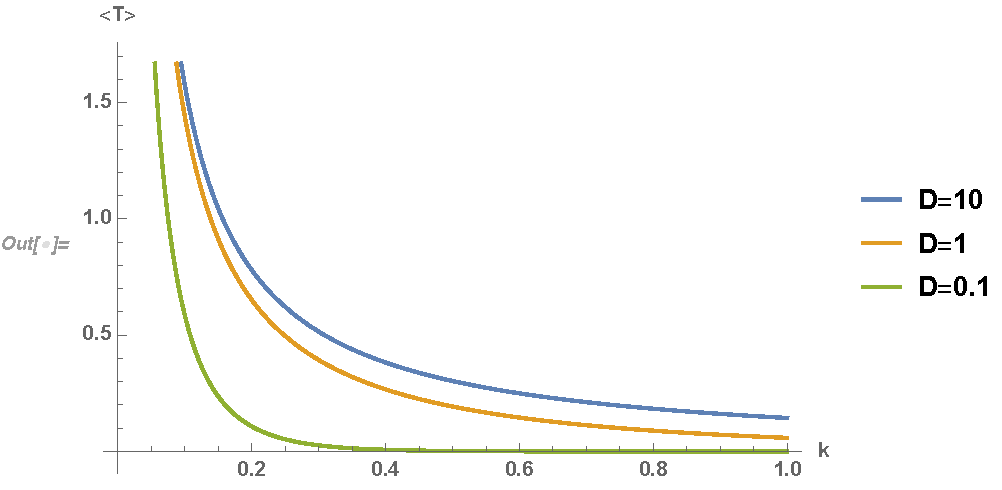
\includegraphics[width=0.5\linewidth]{escape_rate}
	\caption{\small Kramers' escape rate $T(y)$ vs $k$, at different noise levels $D$ from Eq. \ref{eq:OU-ok}.}
	\label{fig:kramers}
\end{figure}

Instead, considering the full potential $U(x) = - px + 1/3 x^3$ generated by a fold normal form $\dot{x} = p - x^2$. It yields an excursion time \citep{Freidlin,Berglund2006} 
\begin{equation}
	\tau_E = \mathcal{O}\left( \exp \left(\frac{2\Delta U}{\sigma^2} \right) \right) \, ,
\end{equation}
 with $\Delta U = U(\sqrt{p}) - U(-\sqrt{p}) = 4/3 p \sqrt{p}$. Excursions are very rare if the noise level is small compared to the time scale separation, $0 < \sigma \ll \sqrt{\epsilon} \ll 1$. If this is not true, random excursions are much more likely and  n-tipping might occur with high chance. \\


Finally, consider a generic double-well potential elicited by a generic bistable function 
\begin{equation}
	dx = f(x) dt + \sigma dW \, .
\end{equation}
Call $\hat{x}_l$ and $\hat{x}_r$ the left and right stable steady-states separated by an unstable potential barrier $\hat{x}_b$. A moving particle subject to noise can exit from its potential well (say, from $\hat{x}_r$) and cross the barrier. When does the first passage occur (on average)? The question is addressed by the exit time. When the first-passage time is averaged over many realizations, we get the mean first-passage time \gls{MFPT}. Let us call $\mathcal{T}(x)$ the MFPT towards $\hat{x}_b$ starting in a generic $x > \hat{x}_b$ (around $a$, if we keep the same image from Fig. \ref{fig:double_well}).  $\mathcal{T}(x)$ satisfies the following diffusion equation \citep{Gardiner1985}:
\begin{equation}
	f(x)\frac{\partial \mathcal{T}(x)}{\partial x} + \frac{1}{2}\sigma \frac{\partial^2 \mathcal{T}(x)}{\partial x^2} = -1
	\label{eq:MFPT}
\end{equation}
given boundary conditions $T(\hat{x}_b) = 0$ and $T(x_{R}) = 0$, where $x_{R}$ denotes the rightmost boundary of the potential well. The \gls{MFPT} is obtained by solving Eq.~\ref{eq:MFPT}.The average passage time from the basin of attraction of $\hat{x}_r$ towards state $\hat{x}_b$ is given by:
\begin{align}
	\nonumber & \mathcal{T}(\hat{x}_r) = 2 \int^{\hat{x}_r}_{\hat{x}_b} \frac{1}{\psi(y)}dy \int^{x_{R}}_y \frac{\psi(z)}{\sigma}dz \\ 
	& \psi(x) = \exp \left(  \int_{x_0}^{x} \frac{2 f(x')}{\sigma} dx' \right)
	\label{eq:MFPT_final}
\end{align}
To estimate the \gls{MFPT} from the leftmost attractor, it suffices to set the boundary conditions appropriately. It is also possible to extend the calculation to non-homogeneous processes and to multi-dimensional domains \citep{Gardiner1985,Arnold1983}.





